\documentclass[11pt]{article}
\usepackage[margin=1in]{geometry}
\usepackage{lmodern}
\usepackage{amsmath,amssymb,amsthm}
\usepackage{graphicx}
\usepackage{booktabs}
\usepackage{microtype}
\usepackage[hidelinks]{hyperref}
\usepackage{xcolor}
\usepackage{mdframed}
\usepackage{caption}
\captionsetup{font=small,labelfont=bf}
\graphicspath{{../figures/}}

\newtheorem{definition}{Definition}
\newtheorem{proposition}{Proposition}
\theoremstyle{remark}
\newtheorem{remark}{Remark}

\newcommand{\Pstar}{P^{*}}
\newcommand{\KL}[2]{D_{\mathrm{KL}}\!\left(#1 \,\middle\|\, #2\right)}
\newcommand{\FB}{\mathcal{F}_{B}}
\newcommand{\Sem}{\mathcal{S}}
\newcommand{\Obs}{\mathcal{O}}

\title{\textbf{Synthetic Semantic Dynamics Under Brand Coherence Field
Theory:\\ A Simulation-Based Technical Report}}
\author{Ricardo Abreu\\
\small Instituto Português de Administração e Marketing de Lisboa (IPAM), Lisbon, Portugal\\
\small \texttt{ricardo.abreu@universidadeeuropeia.pt}}
\date{July 2026}

\begin{document}
\maketitle

\begin{abstract}
\noindent This technical report provides the computational companion to
\emph{Brand Coherence Field Theory} (BCFT), a framework that models brand
meaning as a family of probability distributions over a semantic space and
defines coherence as divergence from an ideal brand distribution
(Abreu, 2026). Whereas the conceptual paper develops the theory and a
simulation \emph{design}, this report supplies the formal apparatus and the
\emph{executed} experiments: explicit divergences, Fisher--Rao geodesics, and
natural-gradient coherence flows on the probability simplex, together with a
fully reproducible Python pipeline and a synthetic dataset. We report three
results. First, coherence declines monotonically with controlled distortion,
and distortion of \emph{core} semantic dimensions is roughly $35\times$ more
costly than distortion of peripheral dimensions. Second, Fisher--Rao geodesics
recover the intrinsic shortest repositioning path exactly, while Euclidean
interpolation is longer and strays measurably from it. Third, the
natural-gradient coherence flow converges geometrically to the ideal
distribution from all tested initial states. The report fixes the canonical
definition of BCFT verbatim so that the conceptual and computational strands
remain locked together. All code, data, and figures are released for
replication.

\medskip
\noindent\textbf{Keywords:} brand coherence; information geometry; Fisher--Rao
metric; Kullback--Leibler divergence; natural gradient; statistical manifold;
reproducible simulation.
\end{abstract}

\section{Introduction and scope}
Brand Coherence Field Theory (BCFT) was introduced as a conceptual framework in
the companion working paper (Abreu, 2026), where the brand is reconceived not as
a fixed bundle of attributes but as a structured field of semantic probability
distributions, and coherence is defined as (negative) divergence from an ideal
brand distribution. That paper deliberately presents the simulation at the level
of \emph{design} and \emph{expected behaviour}, in keeping with its conceptual
contribution and its intended marketing-science audience.

This report is the technical counterpart. Its purpose is narrow and explicit:
to \emph{execute} the BCFT simulation programme with real computation, so that
the formal claims of the theory can be inspected, falsified, and reused. We
make no new empirical claims about real brands here; the data are synthetic by
construction, which is precisely what makes the behaviour of the formalism
transparent. The report contributes (i) a self-contained mathematical
formalization of BCFT on the probability simplex, (ii) reference
implementations of the divergence, geodesic, and natural-gradient machinery,
(iii) three reproducible experiments with real figures and numbers, and (iv) a
synthetic dataset and complete pipeline released for replication.

To keep the conceptual and computational strands of BCFT from drifting apart,
the next section reproduces the theory's canonical definition verbatim before we
formalize it.

\section{The canonical definition of BCFT}
The following statement is reproduced \emph{verbatim} from the companion working
paper (Abreu, 2026, \S3); the present report adopts it without modification.

\begin{mdframed}[backgroundcolor=gray!6,linecolor=gray!40,roundcorner=4pt]
\textbf{Canonical definition.} Brand Coherence Field Theory (BCFT) rests on four
primitives, stated here once and used without modification throughout this paper.
Companion works may develop other formulations of BCFT --- for example a
topological--dynamical formulation over a carrier space --- which share this
definition as their information-geometric special case. (i) \emph{Semantic space}: a brand's possible meanings
are represented in a semantic space, instantiated empirically as expert-coded
categories, topic proportions, or embeddings projected onto the probability
simplex. (ii) \emph{Brand state}: at each observation point $o$ --- a channel,
campaign, stakeholder group, or moment --- the realised meaning of the brand is
a probability distribution $P_o$ over the semantic space. (iii) \emph{Ideal
distribution}: the brand's intended identity is a reference distribution
$\Pstar$ over the same space, estimated from core strategic materials.
(iv) \emph{Coherence}: the coherence of an observed state is
$C(o) = -D(P_o \,\|\, \Pstar)$, the negative divergence of the observed state
from the ideal, where $D$ is a divergence such as the Kullback--Leibler or
Jensen--Shannon divergence. The brand is then a field
$\FB = \{P_o : o \in \Obs\}$ of such states over the set $\Obs$ of relevant
observation points, and coherence is a graded, relational, and measurable
property of that field rather than a binary attribute of the brand as a whole.
In the general three-representation formulation of BCFT, this reference is the
projected identity, and $C(o)$ is the single-reference reduction of a
pairwise-alignment field among projected, perceived, and experienced identities.
\end{mdframed}

\section{Mathematical formalization}
\label{sec:formal}

\subsection{Semantic space and brand states}
Fix a finite semantic space with $K$ dimensions. A brand state is a point of the
$(K-1)$-dimensional probability simplex
\begin{equation}
\Delta^{K-1} = \Big\{ p \in \mathbb{R}^{K} : p_i \ge 0,\ \textstyle\sum_{i=1}^{K} p_i = 1 \Big\}.
\end{equation}
An observation point $o \in \Obs$ (channel, campaign, stakeholder group, moment)
yields a brand state $P_o \in \Delta^{K-1}$; the ideal distribution
$\Pstar \in \Delta^{K-1}$ encodes the intended identity.

\subsection{Coherence as divergence}
For a divergence $D:\Delta^{K-1}\times\Delta^{K-1}\to[0,\infty)$, BCFT coherence
is
\begin{equation}
C(o) = -\,D\!\left(P_o \,\|\, \Pstar\right).
\label{eq:coh}
\end{equation}
We use two divergences. The Kullback--Leibler divergence,
\begin{equation}
\KL{p}{q} = \sum_{i=1}^{K} p_i \log \frac{p_i}{q_i},
\label{eq:kl}
\end{equation}
and the Jensen--Shannon divergence, $\mathrm{JS}(p,q) = \tfrac12\KL{p}{m} +
\tfrac12\KL{q}{m}$ with $m=\tfrac12(p+q)$, which is symmetric and bounded by
$\log 2$. Both belong to the family of $f$-divergences (Csisz\'ar, 1967), and
their local second-order structure is the Fisher information metric below
(Amari \& Nagaoka, 2000).

\subsection{The brand field}
The brand field is the indexed collection
\begin{equation}
\FB = \{P_o : o \in \Obs\},
\label{eq:field}
\end{equation}
so that incoherence can be localized (one channel), clustered (one stakeholder
segment), or diffuse across $\Obs$.

\subsection{Fisher--Rao geometry}
The simplex carries the Fisher--Rao metric, the unique Riemannian metric (up to
scale) invariant under sufficient statistics (Rao, 1945; Chentsov, 1982). Under
the diffeomorphism $s = \sqrt{p}$ (coordinatewise), $\Delta^{K-1}$ maps onto the
positive orthant of the unit sphere $S^{K-1}$, where geodesics are great-circle
arcs. The induced geodesic distance is
\begin{equation}
d_{\mathrm{FR}}(p,q) = 2\arccos\!\Big( \textstyle\sum_{i=1}^{K} \sqrt{p_i q_i} \Big),
\label{eq:frdist}
\end{equation}
the argument being the Bhattacharyya coefficient. The Fisher--Rao geodesic from
$p$ to $q$ is obtained by spherical interpolation of $s=\sqrt{p}$,
\begin{equation}
\gamma(t) = \left( \frac{\sin((1-t)\omega)\,\sqrt{p} + \sin(t\omega)\,\sqrt{q}}{\sin\omega} \right)^{2},
\quad \omega = \arccos\!\big(\textstyle\sum_i \sqrt{p_i q_i}\big),
\label{eq:geo}
\end{equation}
for $t\in[0,1]$, against which we compare the naive Euclidean interpolation
$p^{\mathrm{euc}}(t) = (1-t)p + tq$.

\subsection{Natural-gradient coherence flow}
Coherence-seeking adaptation follows the natural gradient of the divergence with
respect to the Fisher metric (Amari, 2016). On the simplex this yields the
replicator / mirror-descent flow
\begin{equation}
\frac{dp_i}{dt} = -\eta\, p_i \big( g_i - \langle p, g\rangle \big),
\qquad g = \nabla_p\, D\!\left(p \,\|\, \Pstar\right),
\label{eq:flow}
\end{equation}
with step size $\eta>0$. For $D = D_{\mathrm{KL}}$ one has
$g_i = \log(p_i/\Pstar_i)+1$, and the flow keeps $p$ on the simplex and
decreases $\KL{p}{\Pstar}$ monotonically toward its minimum at $p=\Pstar$. The
discrete update used in the experiments is
$p_i \leftarrow p_i \exp(-\eta(g_i - \langle p,g\rangle))$, renormalized.

\begin{proposition}[Fixed point]
$\Pstar$ is the unique fixed point of \eqref{eq:flow} in the interior of
$\Delta^{K-1}$ for $D=D_{\mathrm{KL}}$, and $\KL{p(t)}{\Pstar}$ is
non-increasing along the flow.
\end{proposition}
\noindent The experiments in \S\ref{sec:exp3} confirm this behaviour
numerically (geometric convergence to machine precision).

\section{Synthetic experimental setup}
\label{sec:setup}
We instantiate the running example of the companion paper: a mission-led outdoor
brand with $K=6$ semantic dimensions --- \emph{durability}, \emph{environmental
stewardship}, \emph{repairability}, \emph{functional competence},
\emph{style/aesthetics}, and \emph{status/luxury}. The first four are
\emph{core} (mission/technical); the last two are \emph{peripheral}. The ideal
distribution concentrates mass on the core:
\[
\Pstar = (0.24,\ 0.30,\ 0.20,\ 0.18,\ 0.05,\ 0.03).
\]
Observed states are generated by a controlled perturbation operator that shifts
a fraction (the \emph{perturbation magnitude}) of mass off a chosen set of
dimensions and reallocates it over the complement using a Dirichlet weighting.
All randomness is seeded (\texttt{SEED = 20260628}); the pipeline reproduces
every number and figure below exactly.

\section{Results}

\subsection{Experiment 1 --- divergence and incoherence}
We vary the perturbation magnitude from $0$ to $0.95$ and measure divergence
from $\Pstar$, averaging over $200$ replications per level, separately for core
and peripheral perturbations. Divergence rises monotonically with distortion,
and coherence \eqref{eq:coh} declines correspondingly
(Figure~\ref{fig:exp1}). Crucially, the cost of distortion is
structurally weighted: at maximum magnitude, core distortion produces
$\KL{P_o}{\Pstar} \approx 2.40$ against $\approx 0.069$ for peripheral
distortion --- a ratio of about $\mathbf{34.8\times}$. BCFT therefore captures
that not all deviations are equally damaging; movement away from core meanings
is far more incoherent than equivalent movement in peripheral style cues.

\begin{figure}[ht]
\centering
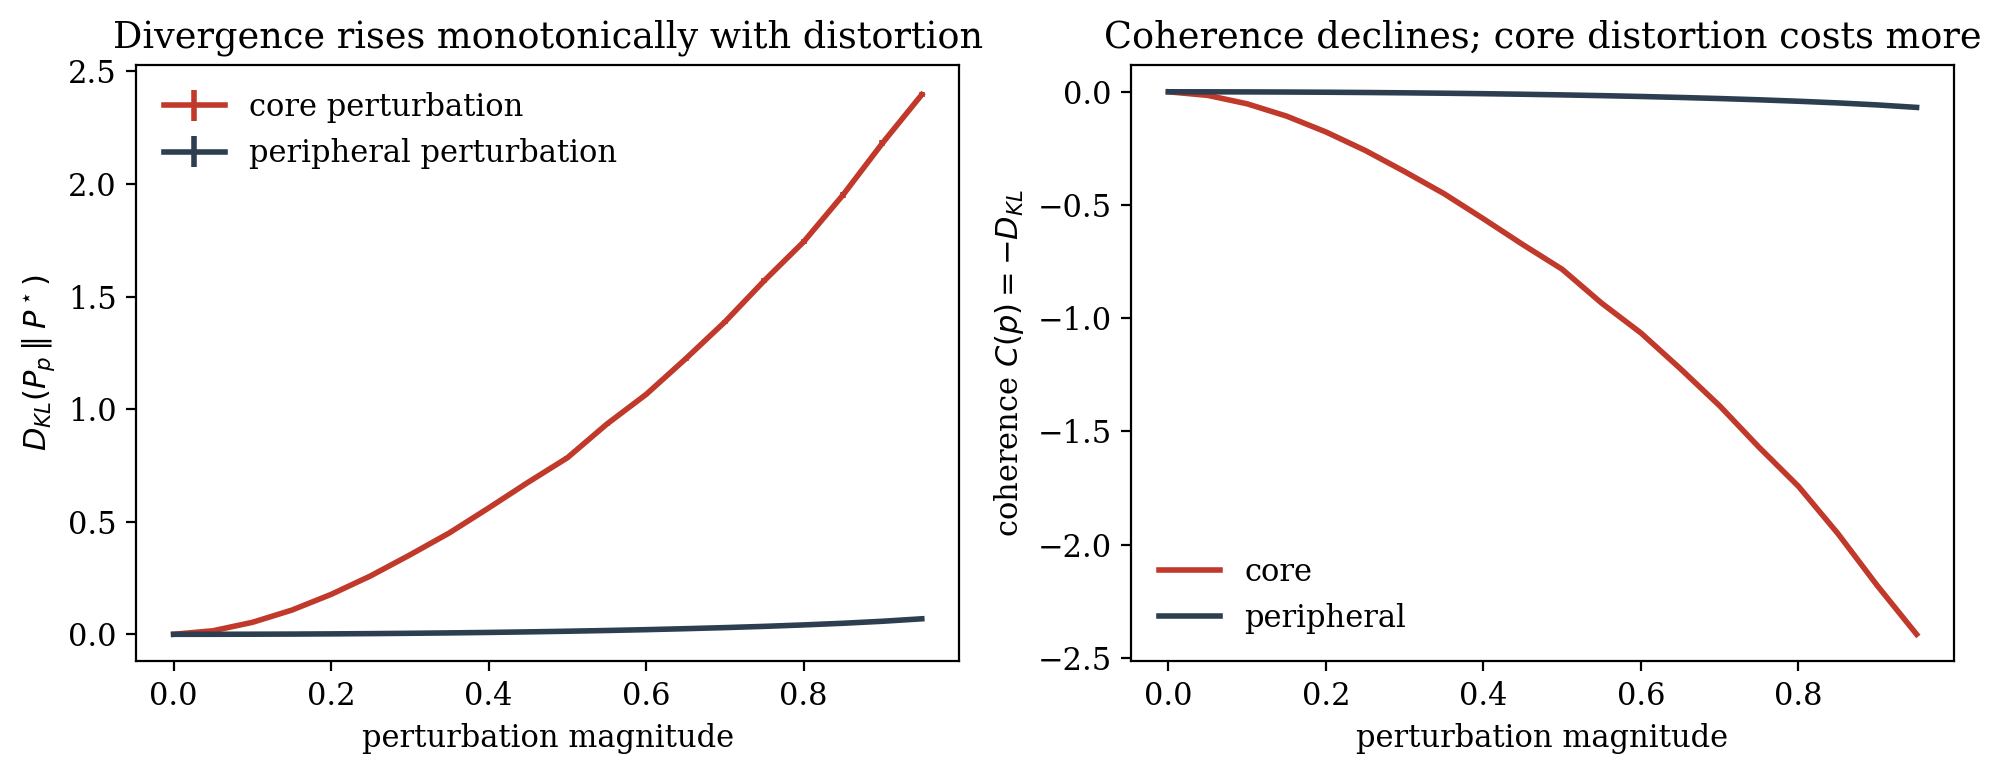
\includegraphics[width=\linewidth]{fig_exp1_monotonic.png}
\caption{Experiment 1. Left: Kullback--Leibler divergence from the ideal rises
monotonically with perturbation magnitude, steeply for core distortion and
weakly for peripheral distortion. Right: the corresponding coherence
$C(o)=-D_{\mathrm{KL}}$. Error bars are standard errors over 200 replications.}
\label{fig:exp1}
\end{figure}

\subsection{Experiment 2 --- geodesic versus Euclidean movement}
We compare repositioning from a core-heavy state $(0.80,0.15,0.05)$ to a
status-heavy state $(0.05,0.15,0.80)$ on the $K=3$ simplex, under the
Fisher--Rao geodesic \eqref{eq:geo} and under Euclidean interpolation
(Figure~\ref{fig:exp2}). The geodesic length equals the Fisher--Rao distance
\eqref{eq:frdist} to numerical precision ($1.9769$ vs.\ $1.9769$), validating
the implementation. The Euclidean path is longer ($1.9930$, an excess of
$\mathbf{0.81\%}$) and, more importantly, traverses \emph{different}
intermediate brand states: the maximum Fisher--Rao deviation between the two
paths at equal interpolation parameter is $\mathbf{0.120}$. The shortest path in
a flat projection is thus not the intrinsically shortest --- nor the same ---
trajectory of semantic change, which is the strategic intuition BCFT formalizes.

\begin{figure}[ht]
\centering
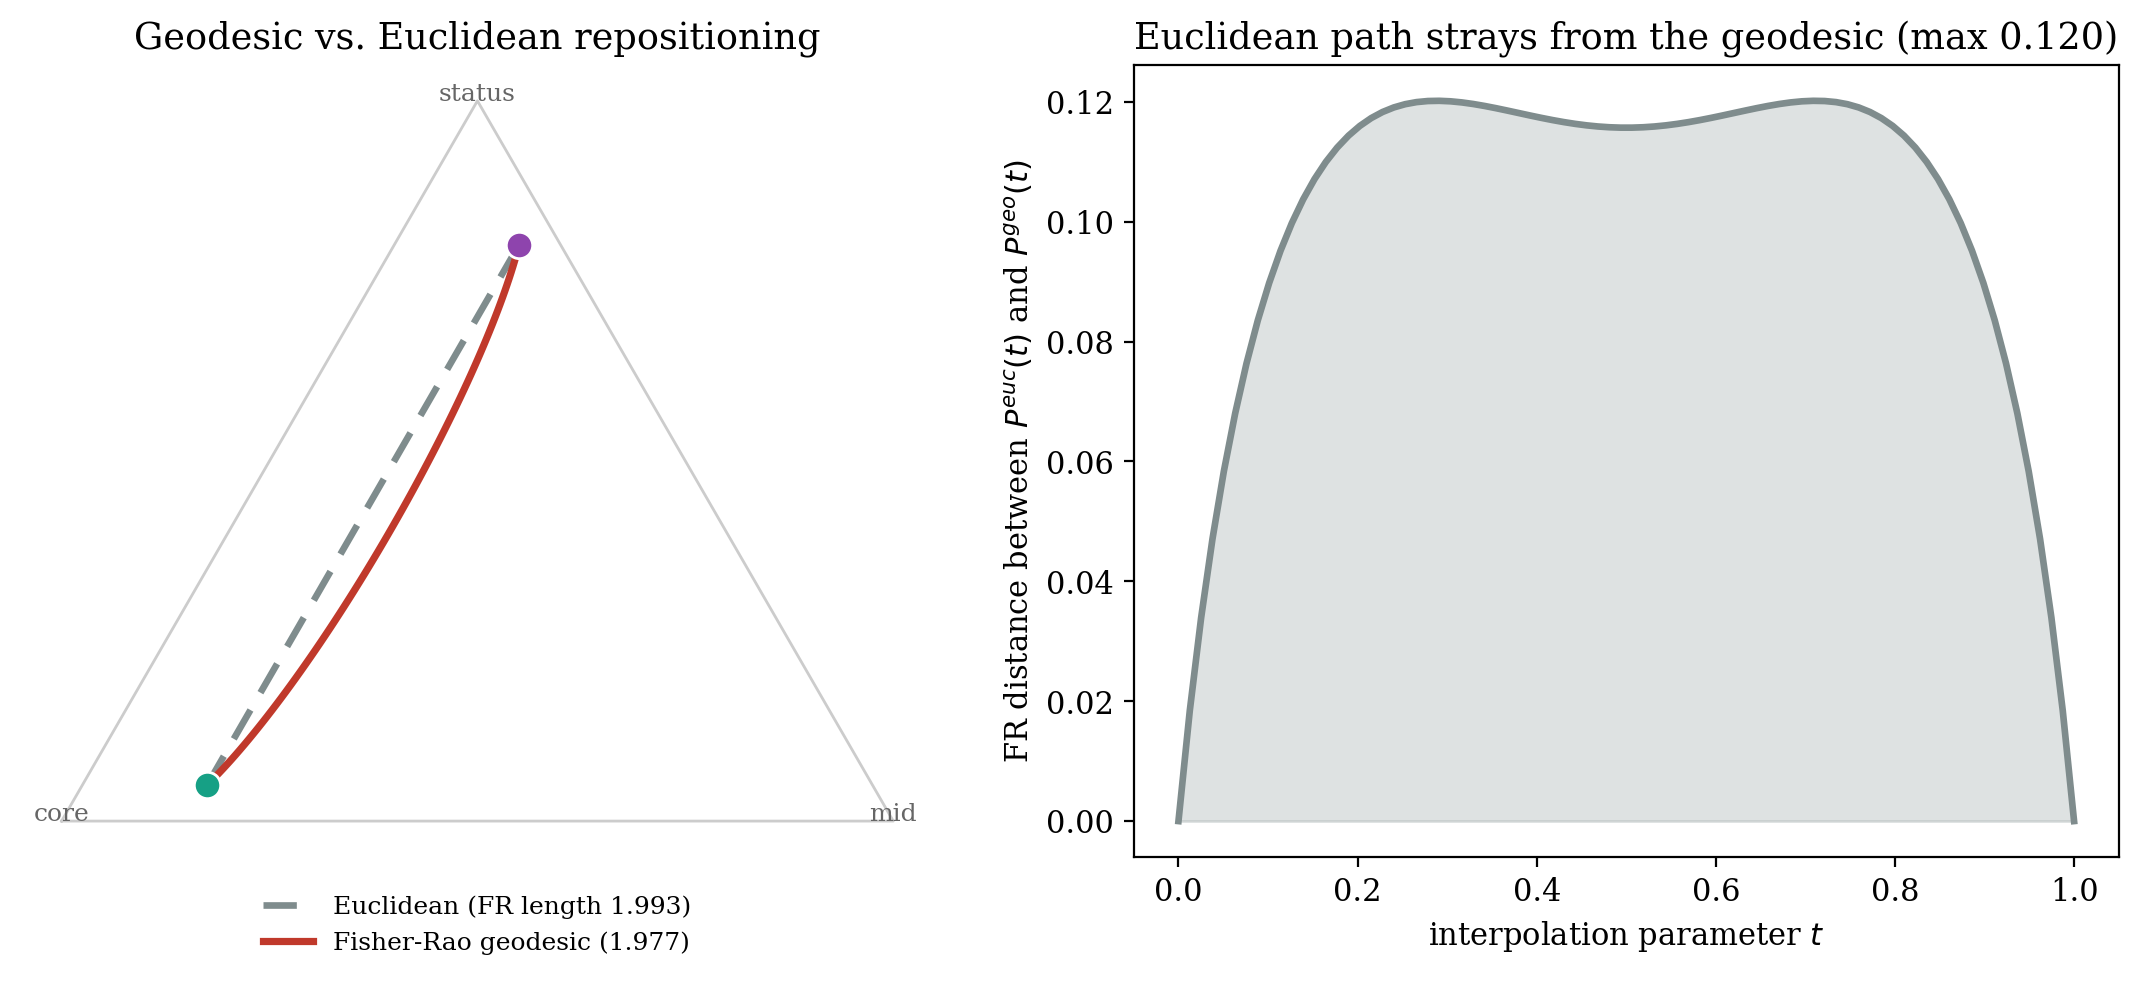
\includegraphics[width=\linewidth]{fig_exp2_geodesic.png}
\caption{Experiment 2. Left: on the 3-dimensional simplex, the Fisher--Rao
geodesic (solid) bows away from the Euclidean chord (dashed). Right: the
Fisher--Rao distance between the Euclidean and geodesic states at the same
interpolation parameter $t$, peaking at $0.120$.}
\label{fig:exp2}
\end{figure}

\subsection{Experiment 3 --- convergent coherence flows}
\label{sec:exp3}
We initialise the natural-gradient flow \eqref{eq:flow} from six random states
and run it toward $\Pstar$ with $\eta=0.25$ for $150$ iterations
(Figure~\ref{fig:exp3}). All trajectories converge geometrically; the largest
final divergence across runs is $\approx 1.4\times10^{-16}$ (machine precision),
confirming the fixed-point proposition. A $K=3$ projection shows the
trajectories descending onto the ideal. This operationalizes BCFT's notion of
\emph{semantic repair}: corrective communication that follows the geometry of
the semantic space restores coherence efficiently.

\begin{figure}[ht]
\centering
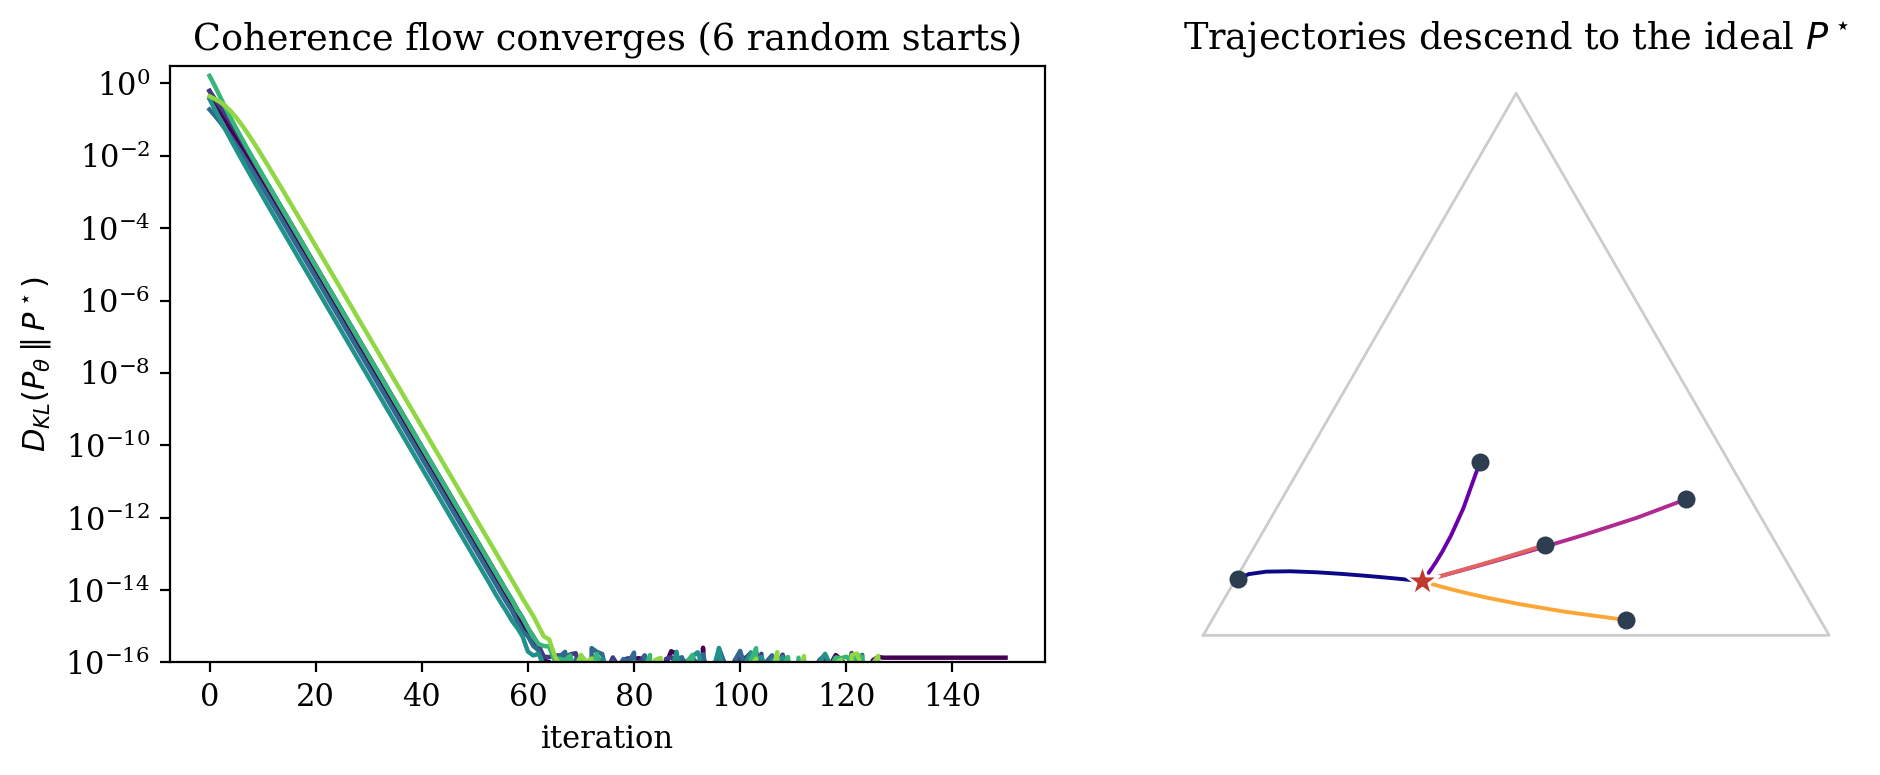
\includegraphics[width=\linewidth]{fig_exp3_flow.png}
\caption{Experiment 3. Left: $D_{\mathrm{KL}}(P_\theta\|\Pstar)$ on a log scale
for six random initializations; all converge to machine precision. Right: a
ternary projection of trajectories descending to the ideal $\Pstar$ (star).}
\label{fig:exp3}
\end{figure}

\subsection{Synthetic brand-field dataset}
For downstream replication we release a synthetic brand field of $100$
observations across four source types (institutional, campaign, reviews,
lifestyle), each generated by perturbing $\Pstar$ with source-specific
magnitude and recording the full distribution together with its KL, JS, and
Fisher--Rao distances to the ideal and its coherence. Table~\ref{tab:summary}
collects the headline quantities of all three experiments.

\begin{table}[ht]
\centering
\caption{Headline results (seed 20260628).}
\label{tab:summary}
\small
\begin{tabular}{lll}
\toprule
Experiment & Quantity & Value \\
\midrule
1 & KL monotonic in distortion (core) & yes \\
1 & KL at max distortion, core & $2.396$ \\
1 & KL at max distortion, peripheral & $0.069$ \\
1 & core/peripheral cost ratio & $34.8\times$ \\
2 & Fisher--Rao distance (endpoints) & $1.9769$ \\
2 & geodesic length $=$ FR distance & yes ($1.9769$) \\
2 & Euclidean path length & $1.9930$ ($+0.81\%$) \\
2 & max FR deviation (Euclidean vs geodesic) & $0.120$ \\
3 & natural-gradient flow converges (6 starts) & yes \\
3 & max final $D_{\mathrm{KL}}$ & $1.4\times10^{-16}$ \\
\bottomrule
\end{tabular}
\end{table}

\section{Discussion and limitations}
The experiments demonstrate the internal coherence and computational
tractability of BCFT, not its empirical validity. Three limitations follow
directly from the synthetic design. First, the semantic space here is
stipulated; in application the choice of dimensions and the estimation of
$\Pstar$ are substantive modelling decisions that will shape coherence profiles.
Second, divergence choice matters: KL and JS encode different sensitivities, and
results may shift under other $f$-divergences or under the Wasserstein geometry,
which is non-invariant but metric on the sample space (Amari, 2021). Third,
the natural-gradient flow is shown to converge for the convex KL objective;
richer objectives --- for example multi-ideal or mixture coherence --- may
exhibit local traps, which we leave to future work. These constructions are now
computationally accessible through general-purpose information-geometry tooling
(Le Brigant et al., 2023), and the present pipeline is designed to extend to
them. The empirical programme --- estimating $P_o$ from real brand text along
the lines of computational brand-image work (Mitra \& Jenamani, 2020; Ranfagni
et al., 2021) --- is the subject of the separate empirical paper.

\section*{Reproducibility statement}
All results are produced by the released pipeline. The core library
(\texttt{src/bcft.py}) implements the divergences, Fisher--Rao distance,
geodesic, and natural-gradient flow; \texttt{src/run\_experiments.py}
regenerates every figure, the synthetic dataset, and the results summary from a
single fixed seed. See \texttt{README.md} for environment and execution
instructions; \texttt{requirements.txt} pins dependencies. The repository is
intended for archival on Zenodo with a citable DOI.

\section*{References}
\small
\begin{itemize}\setlength\itemsep{1pt}
\item[] Abreu, R. (2026). \emph{Brand Coherence Field Theory: An
information-geometric framework for modelling brand meaning}. Working paper
(companion conceptual paper).
\item[] Amari, S. (2016). \emph{Information geometry and its applications}.
Tokyo: Springer. \texttt{https://doi.org/10.1007/978-4-431-55978-8}
\item[] Amari, S. (2021). Information geometry. \emph{Japanese Journal of
Mathematics}, 16, 1--48. \texttt{https://doi.org/10.1007/s11537-020-1920-5}
\item[] Amari, S., \& Nagaoka, H. (2000). \emph{Methods of information
geometry}. Providence, RI: American Mathematical Society.
\item[] Chentsov, N. N. (1982). \emph{Statistical decision rules and optimal
inference}. Providence, RI: American Mathematical Society.
\item[] Csisz\'ar, I. (1967). Information-type measures of difference of
probability distributions and indirect observation. \emph{Studia Scientiarum
Mathematicarum Hungarica}, 2, 299--318.
\item[] Le Brigant, A., Deschamps, J., Collas, A., \& Miolane, N. (2023).
Parametric information geometry with the package Geomstats. \emph{ACM
Transactions on Mathematical Software}, 49(4), 1--26.
\texttt{https://doi.org/10.1145/3627538}
\item[] Mitra, S., \& Jenamani, M. (2020). OBIM: A computational model to
estimate brand image from online consumer review. \emph{Journal of Business
Research}, 114, 213--226.
\texttt{https://doi.org/10.1016/j.jbusres.2020.04.003}
\item[] Ranfagni, S., Faraoni, M., Zollo, L., \& Vannucci, V. (2021). Combining
online market research methods for investigating brand alignment: The case of
Nespresso. \emph{British Food Journal}, 123(13), 37--58.
\texttt{https://doi.org/10.1108/BFJ-06-2020-0462}
\item[] Rao, C. R. (1945). Information and the accuracy attainable in the
estimation of statistical parameters. \emph{Bulletin of the Calcutta
Mathematical Society}, 37, 81--91.
\end{itemize}

\end{document}
